
%% bare_jrnl_compsoc.tex
%% V1.4a
%% 2014/09/17
%% by Michael Shell
%% See:
%% http://www.michaelshell.org/
%% for current contact information.
%%
%% This is a skeleton file demonstrating the use of IEEEtran.cls
%% (requires IEEEtran.cls version 1.8a or later) with an IEEE
%% Computer Society journal paper.
%%
%% Support sites:
%% http://www.michaelshell.org/tex/ieeetran/
%% http://www.ctan.org/tex-archive/macros/latex/contrib/IEEEtran/
%% and
%% http://www.ieee.org/

%%*************************************************************************
%% Legal Notice:
%% This code is offered as-is without any warranty either expressed or
%% implied; without even the implied warranty of MERCHANTABILITY or
%% FITNESS FOR A PARTICULAR PURPOSE! 
%% User assumes all risk.
%% In no event shall IEEE or any contributor to this code be liable for
%% any damages or losses, including, but not limited to, incidental,
%% consequential, or any other damages, resulting from the use or misuse
%% of any information contained here.
%%
%% All comments are the opinions of their respective authors and are not
%% necessarily endorsed by the IEEE.
%%
%% This work is distributed under the LaTeX Project Public License (LPPL)
%% ( http://www.latex-project.org/ ) version 1.3, and may be freely used,
%% distributed and modified. A copy of the LPPL, version 1.3, is included
%% in the base LaTeX documentation of all distributions of LaTeX released
%% 2003/12/01 or later.
%% Retain all contribution notices and credits.
%% ** Modified files should be clearly indicated as such, including  **
%% ** renaming them and changing author support contact information. **
%%
%% File list of work: IEEEtran.cls, IEEEtran_HOWTO.pdf, bare_adv.tex,
%%                    bare_conf.tex, bare_jrnl.tex, bare_conf_compsoc.tex,
%%                    bare_jrnl_compsoc.tex, bare_jrnl_transmag.tex
%%*************************************************************************


% *** Authors should verify (and, if needed, correct) their LaTeX system  ***
% *** with the testflow diagnostic prior to trusting their LaTeX platform ***
% *** with production work. IEEE's font choices and paper sizes can       ***
% *** trigger bugs that do not appear when using other class files.       ***                          ***
% The testflow support page is at:
% http://www.michaelshell.org/tex/testflow/


\documentclass[10pt,conference,onecolumn,compsoc]{IEEEtran}


\usepackage{hyperref}
\usepackage{enumitem}
\setlist[itemize]{leftmargin=3 cm}
\setlist[enumerate]{leftmargin=3cm}



% *** CITATION PACKAGES ***
%
\ifCLASSOPTIONcompsoc
  % IEEE Computer Society needs nocompress option
  % requires cite.sty v4.0 or later (November 2003)
  \usepackage[nocompress]{cite}
\else
  % normal IEEE
  \usepackage{cite}
\fi
% cite.sty was written by Donald Arseneau
% V1.6 and later of IEEEtran pre-defines the format of the cite.sty package
% \cite{} output to follow that of IEEE. Loading the cite package will
% result in citation numbers being automatically sorted and properly
% "compressed/ranged". e.g., [1], [9], [2], [7], [5], [6] without using
% cite.sty will become [1], [2], [5]--[7], [9] using cite.sty. cite.sty's
% \cite will automatically add leading space, if needed. Use cite.sty's
% noadjust option (cite.sty V3.8 and later) if you want to turn this off
% such as if a citation ever needs to be enclosed in parenthesis.
% cite.sty is already installed on most LaTeX systems. Be sure and use
% version 5.0 (2009-03-20) and later if using hyperref.sty.
% The latest version can be obtained at:
% http://www.ctan.org/tex-archive/macros/latex/contrib/cite/
% The documentation is contained in the cite.sty file itself.



% *** GRAPHICS RELATED PACKAGES ***
%
\ifCLASSINFOpdf
   \usepackage[pdftex]{graphicx}
 
\else
 
\fi
% graphicx was written by David Carlisle and Sebastian Rahtz. It is
% required if you want graphics, photos, etc. graphicx.sty is already
% installed on most LaTeX systems. The latest version and documentation
% can be obtained at: 
% http://www.ctan.org/tex-archive/macros/latex/required/graphics/
% Another good source of documentation is "Using Imported Graphics in
% LaTeX2e" by Keith Reckdahl which can be found at:
% http://www.ctan.org/tex-archive/info/epslatex/
%
% latex, and pdflatex in dvi mode, support graphics in encapsulated
% postscript (.eps) format. pdflatex in pdf mode supports graphics
% in .pdf, .jpeg, .png and .mps (metapost) formats. Users should ensure
% that all non-photo figures use a vector format (.eps, .pdf, .mps) and
% not a bitmapped formats (.jpeg, .png). IEEE frowns on bitmapped formats
% which can result in "jaggedy"/blurry rendering of lines and letters as
% well as large increases in file sizes.
%
% You can find documentation about the pdfTeX application at:
% http://www.tug.org/applications/pdftex









% *** PDF, URL AND HYPERLINK PACKAGES ***
%
\usepackage{url}
% url.sty was written by Donald Arseneau. It provides better support for
% handling and breaking URLs. url.sty is already installed on most LaTeX
% systems. The latest version and documentation can be obtained at:
% http://www.ctan.org/tex-archive/macros/latex/contrib/url/
% Basically, \url{my_url_here}.




\begin{document}

\title{Music Manager}
%
%

% received ..."  text while in non-compsoc journals this is reversed. Sigh.

\author{Andrew Marshall, Kyle Rolland\\% <-this % stops a space
}

\IEEEtitleabstractindextext{%
\begin{abstract}
The goal of this project is to create an interface that allows a user to store and manage music on their machine. Users will be able to create play lists, favorite certain songs, and sort songs by the artist, or the song name. Our goal with this project is to make a simple version of music applications like Spotify or iTunes, for people who don't like using their current music player application.
\end{abstract}

}


% make the title area
\maketitle



\IEEEdisplaynontitleabstractindextext

\IEEEpeerreviewmaketitle



\section{Introduction}


Music is an everyday part of life, and many people go everyday without even thinking about the luxury that we have in the modern era, being able to listen to what we want, wherever we want to. Following this, there are many many platforms that one can use to access music. We aim to reproduce one such platform, creating an interface that allows someone to add music of their choosing, organize it, and play it. 
	
Providing people with more options is never a bad thing. Even if there are only a few things that differentiate one software from another, there are always going to be users looking for new experiences. We would like to be able to appeal to as wide an audience as possible, people who have problems with the existing flaws in other software, which are ignored or put off of being fixed by developers. Helping those people find a new place where they feel they can store their favorite songs can make a large difference, especially because music can be a very valuable, memorable resource for some people.

\subsection{Background}
Over the course of this proposal, we will use the term Metadata, and in this case, it's really just a technical term for basic music information. It pertains to things like album art, release date, track/song length, genre, artist, and the songs title.

We decided on a project like this because music is something that is easy to make connections between. Thankfully, The two of us had common ground in a genre that we used to listen to, but even if we didn't, it would be easy to come together to work on a project like this. It originally sprouted as an idea for an audio waveform visualizer, the flashing bars/lights that you'll see with music videos, that correspond to the beat of the song, or the lyrics. Neither of us have looked into what it takes to make those, and some further consideration led us to decide that it would be better to take a step back and just make a music management interface.

Andrew has run into problems with CDs on iTunes, so we hope to be able to implement a way transfer music from the manager to the CD, allowing the manager to effectively use and read CDs.

Kyle's main music application is Apple Music , and he has some issues with listening queue management, for example, shuffling a play list, and then adding it to the end of the list of what is currently being listened to, which is not possible in the application. If we could work the capability into this project, it may become an alternative listening application for him as well.

\subsection{Impacts}
There are many music managing systems on the internet, and we would like to see if we can create something worth telling others about, so that they can use as well. We want to add some functionality that gives us a chance to stand out, making it easier to reach even just a few people, and give them another place to handle the songs that they hold dear. It doesn't take much to brighten someone's day, and hopefully with this project we can manage to do that for a handful of people.

\subsection{Challenges}
It may be difficult to organize and handle the previously mentioned metadata, since there is a lot of information that goes along with it. We also may run into trouble trying to create a system to accept different file types, like .mp3 versus .mp4 versus .wav, but working a system like this out would prove very useful for attracting more users. Making a display for things like album art, and giving the user the option to upload their own art to go with songs or created play lists may also prove to be difficult, partially because of accepting images, and partially reaching back to accepting different image file types, like .jpeg and .png. Lastly, we are still sort of hoping to implement an audio waveform visualizer somewhere within the interface, and we think this will prove to be the biggest hurdle, especially if we can't find a framework to start with.


\section{Scope}
Our project will be completed when we have an interface that allows the user to add songs of their choosing, modify their metadata, add those songs to play lists and edit those play lists freely and easily, search for songs within their database, and sort them by given data types, like artist, genre, and song title

We have some ideas for stretch goals. One of them would be implementing the previously mentioned audio waveform visualizer. Along with this, being able to easily export your play lists or songs to various different platforms would be very handy. Lastly, we would love to be able to implement a system that allows the user to upload images for artwork that will display when a song is playing, be it album art, or an image that will act as the cover of a given play list, allowing for more user customization.

\subsection{Requirements}

\subsubsection{Functional}
\begin{itemize}
\item Store songs that are currently being played, and are queued to play
\item Keep track of previously played songs for accessibility later
\item Display current song being played, as well as associated artwork
\item Hold songs that are being played for storage across listening sessions
\item Give access to music metadata so user can change it
\item Allow for customization of user created play lists
\item Prevent duplication of music in library
\item Adhere to copyright laws, recognizing proper credit to musicians 
\end{itemize}

\subsubsection{Non-Functional}
\begin{itemize}
\item When user updates music information, update within 5 seconds
\item Ensure that music and image files are of proper formatting
\item Ensure that songs and data are easily accessible and understandable to the user, through effective use of application interface
\end{itemize}

\subsection{Use Cases}
Use Case index can be seen in Table \ref{tab:useCaseIndex}.




\begin{table}
\centering
\begin{tabular}{|c|c|c|c|c|}
\hline
Use Case ID & Use Case Name & Primary Actor & Complexity & Priority \\
\hline \hline
1 & Add song to queue & Listener & Med & 1\\
\hline
2 & Add new song to manager & Listener & Hard & 1\\
\hline
3 & Add album art & Listener & Med & 2\\
\hline
4 & Play from CD & Listener & Hard & 3\\
\hline
5 & Change volume & Listener & Med & 1\\
\hline

\end{tabular}
\caption{Use case index}
\label{tab:useCaseIndex}
\end{table}


\begin{itemize}
\item[Use Case Number:] 1
\item[Use Case Name:] Add song to queue
\item[Description:] User selects a song that they wish to play next. They will click on a plus button that appears when hovering over the song. This will add the song to the list, and will be played next.
\end{itemize}

\begin{enumerate}
\item User selects song that they want to play next
\item After selecting song, plus button appears on song bar
\item User presses button, adds song to queue
\item[Termination Outcome:] Selected song will be played next
\end{enumerate}

(see Figure \ref{AddSong})

\begin{itemize}
\item[Use Case Number:] 2
\item[Use Case Name:] Add music to manager
\item[Description:] Menu bar at top of screen will have a file button. User presses button, and asks user what they would like to add. User selects song, asks for file name of song that will be added. If file can be found, and is an accepted file type, it will be added to the manager.
\end{itemize}

\begin{enumerate}
\item User presses File button on menu bar
\item Drop down menu appears, allows user to click on Add Song...
\item User enters song file that they want to add
\item If file is appropriate formatting, song is added to manager
\item [Termination Outcome:] New song is present in management library
\end{enumerate}

Alternatively:
\begin{enumerate}
\item User presses File button on menu bar
\item Drop down menu appears, allows user to click Add Song...
\item User enters song file that they want to add
\item Song is already in library
\item Song is prevented from being added
\item (OPTIONAL: Sends user to song in library once prevention occurs)
\item [Termination Outcome:] Duplication of song(s) prevented
\end{enumerate}

(see Figure \ref{AddSong})

\begin{itemize}
\item[Use Case Number:] 3
\item[Use Case Name:] Add album art
\item[Description:] When looking at an album or play list, displays a button that will allow the user to select an image to upload. Once selected, image will be used as art for the given album/play list.
\end{itemize}

\begin{enumerate}
\item User opens album or play list
\item User presses button at top corner of album art area
\item Menu appears that allows user to modify item
\item User selects Add Image...
\item User enters image name that they would like
\item If file is appropriate formatting, art is replaced
\item [Termination Outcome:] Previous album art is replaced with new art
\end{enumerate}

(see Figure \ref{AddAlbumArt})

\begin{itemize}
\item[Use Case Number:] 4
\item[Use Case Name:] Play from CD
\item[Description:] Menu bar at top of screen will have a device button, clicking on it allows user to select an outside device to play music from, or send music to (This is just a goal for right now, something to work towards).
\end{itemize}

\begin{enumerate}
\item User presses Device button on menu bar
\item Drop down menu appears
\item User selects Import from CD
\item Music on CD is loaded into manager
\item [Termination Outcome:] Music present on CD is now loaded into user's library
\end{enumerate}

(See Figure \ref{PlayCD})

\begin{itemize}
\item[Use Case Number:] 5
\item[Use Case Name:] Change volume
\item[Description:] Volume buttons displayed beneath play section (Possibly replace with volume slider/better display). User presses + button to increment volume up by one, and - button to decrement volume by one, to an upper and lower limit respectfully.
\end{itemize}

\begin{enumerate}
\item User presses plus button next to speaker image
\item [Termination Outcome:] Volume increases by one increment
\end{enumerate}

Alternatively:
\begin{enumerate}
\item User presses minus button next to speaker image
\item [Termination Outcome:] Volume decreases by one increment
\end{enumerate}

(See Figure \ref{VolumeButton})

You will then need to continue to flesh out all use cases you have identified for your project.

\subsection{Interface Mockups}

\begin{figure}[ht!]
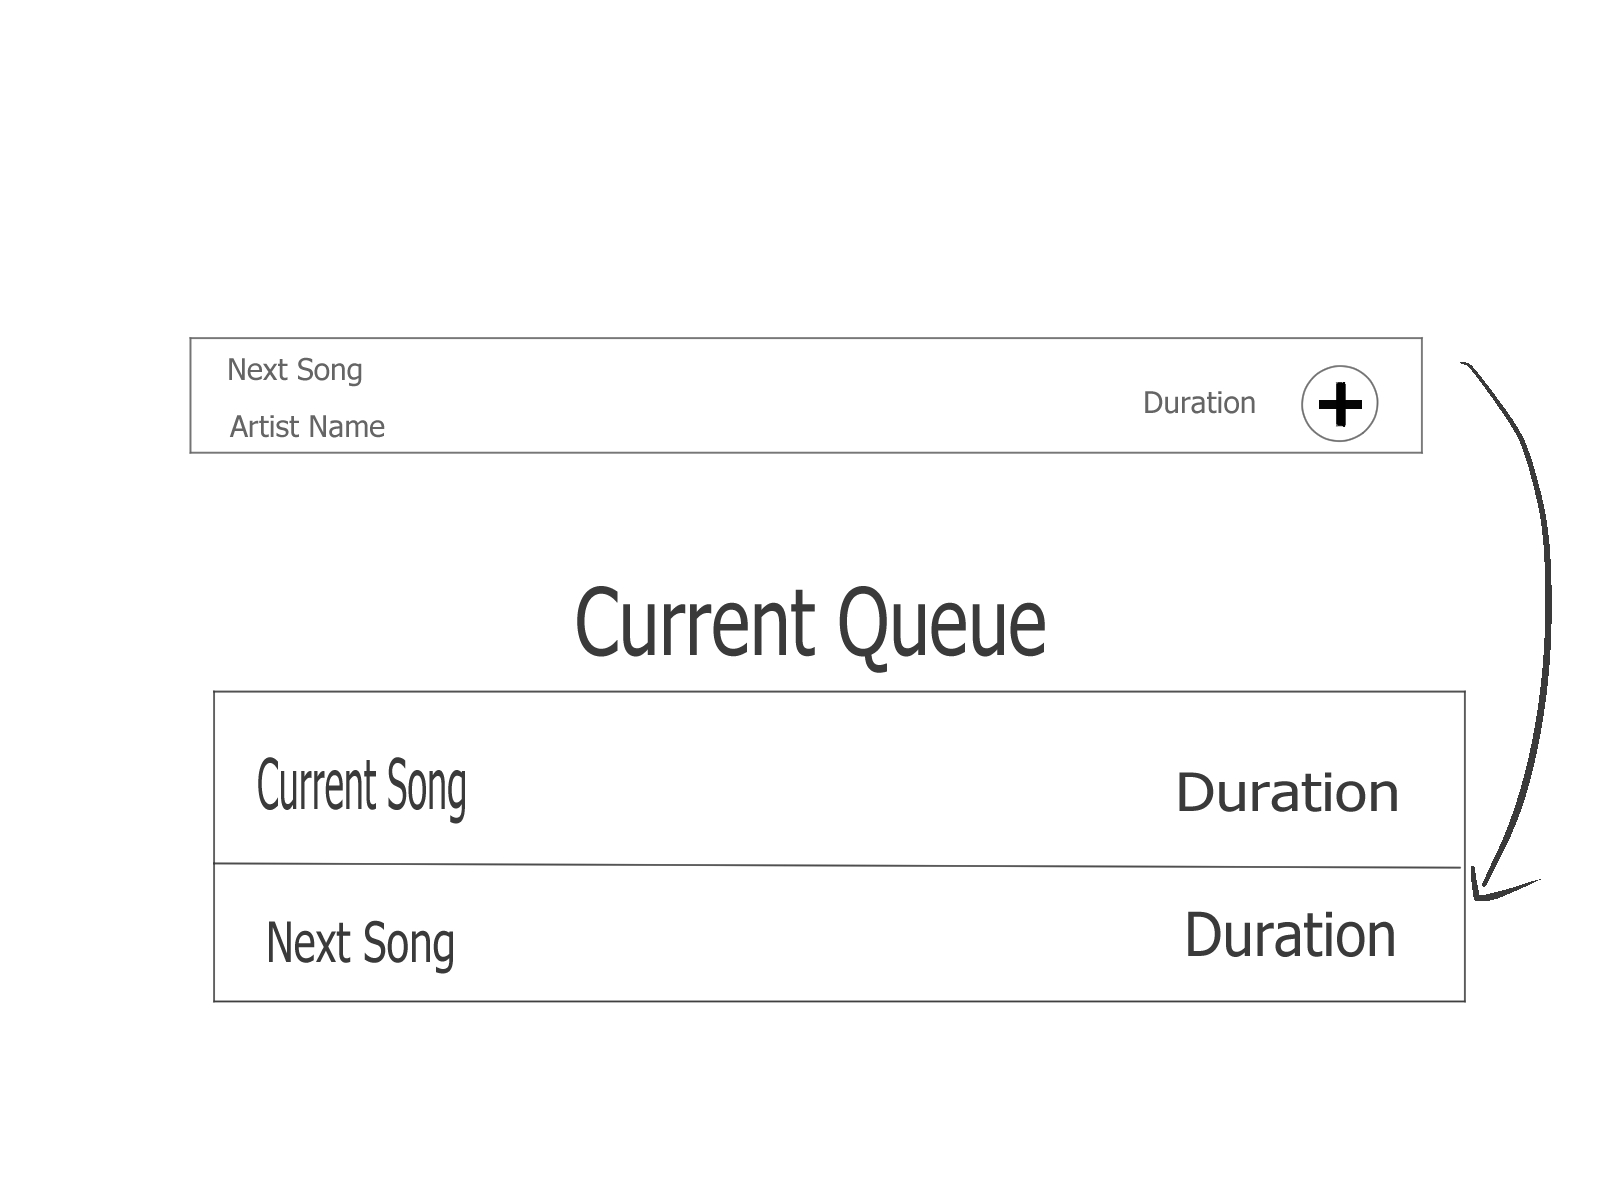
\includegraphics[height=250px, width=350px]{Add_Song_Queue_Mock_Up.jpg}
\caption{Use Case 1, Adding song to queue}
\label{AddSong}
\end{figure}

\begin{figure}[ht!]
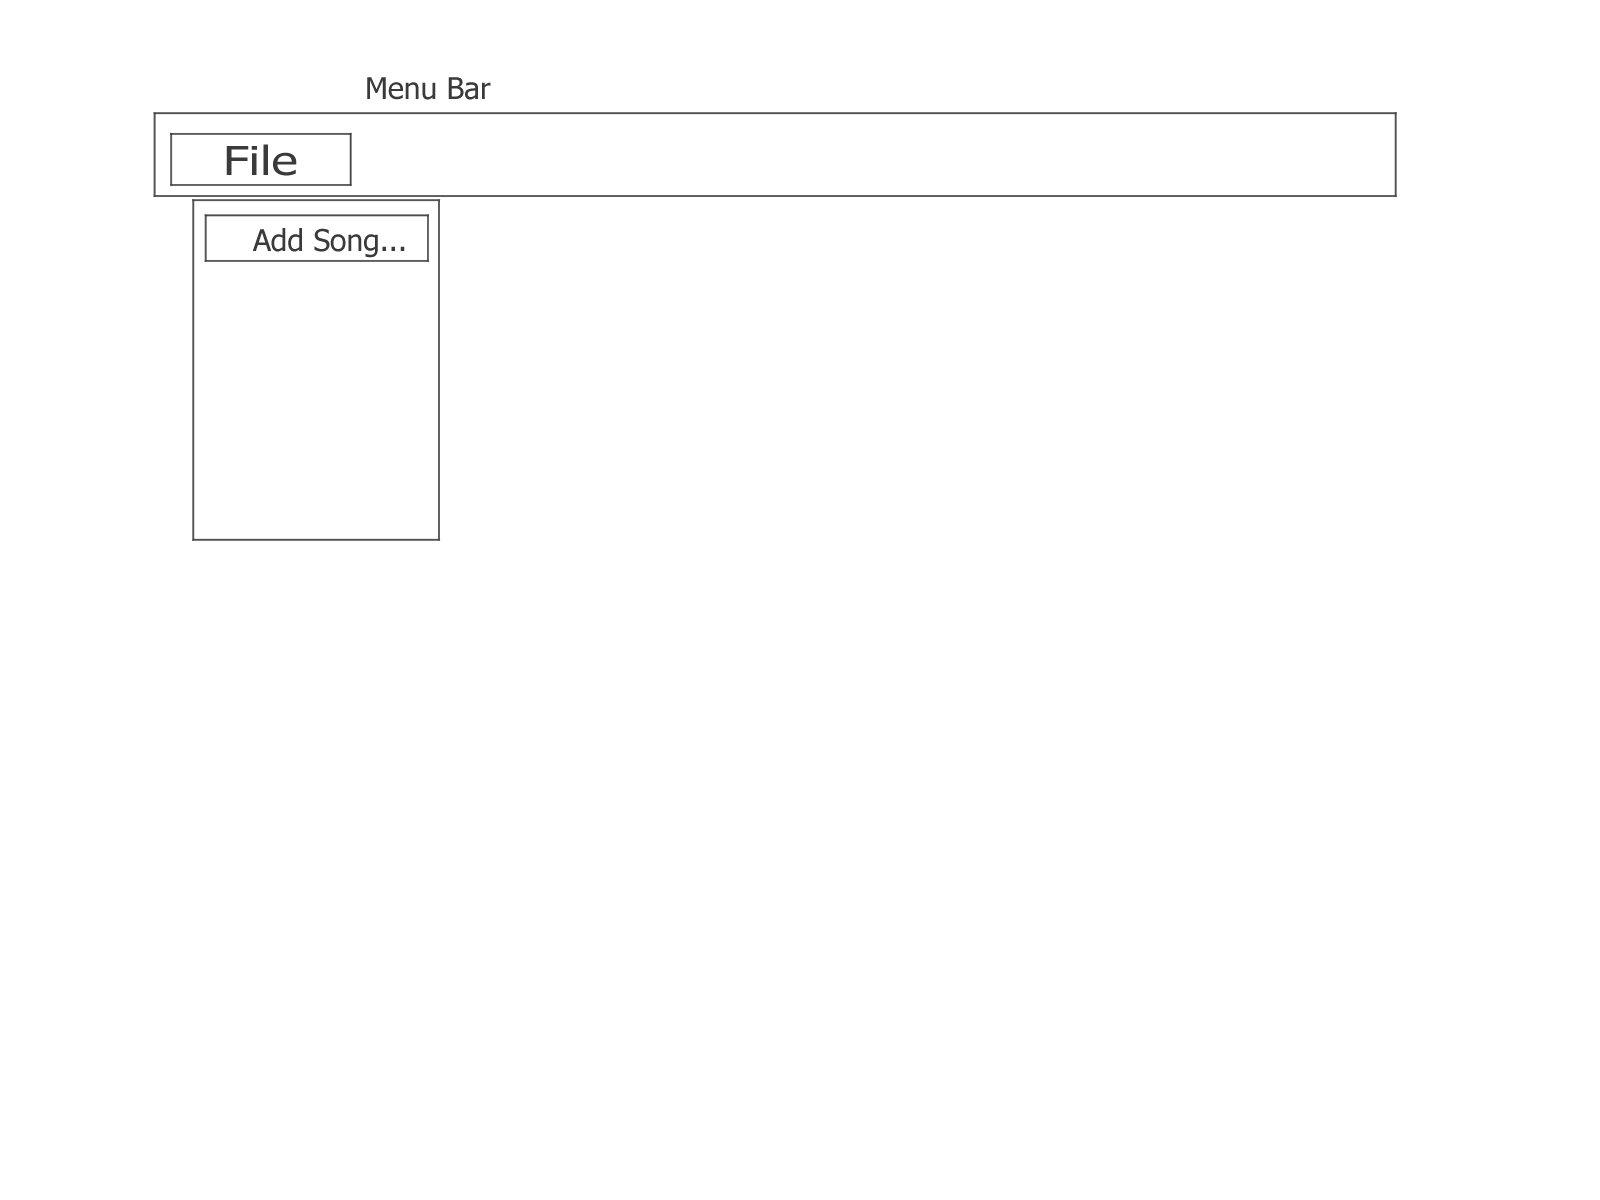
\includegraphics[height=250px, width=350px]{Add_Music_Mock_Up.jpg}
\caption{Use Case 2, Adding music to manager}
\label{AddMusic}
\end{figure}

\begin{figure}
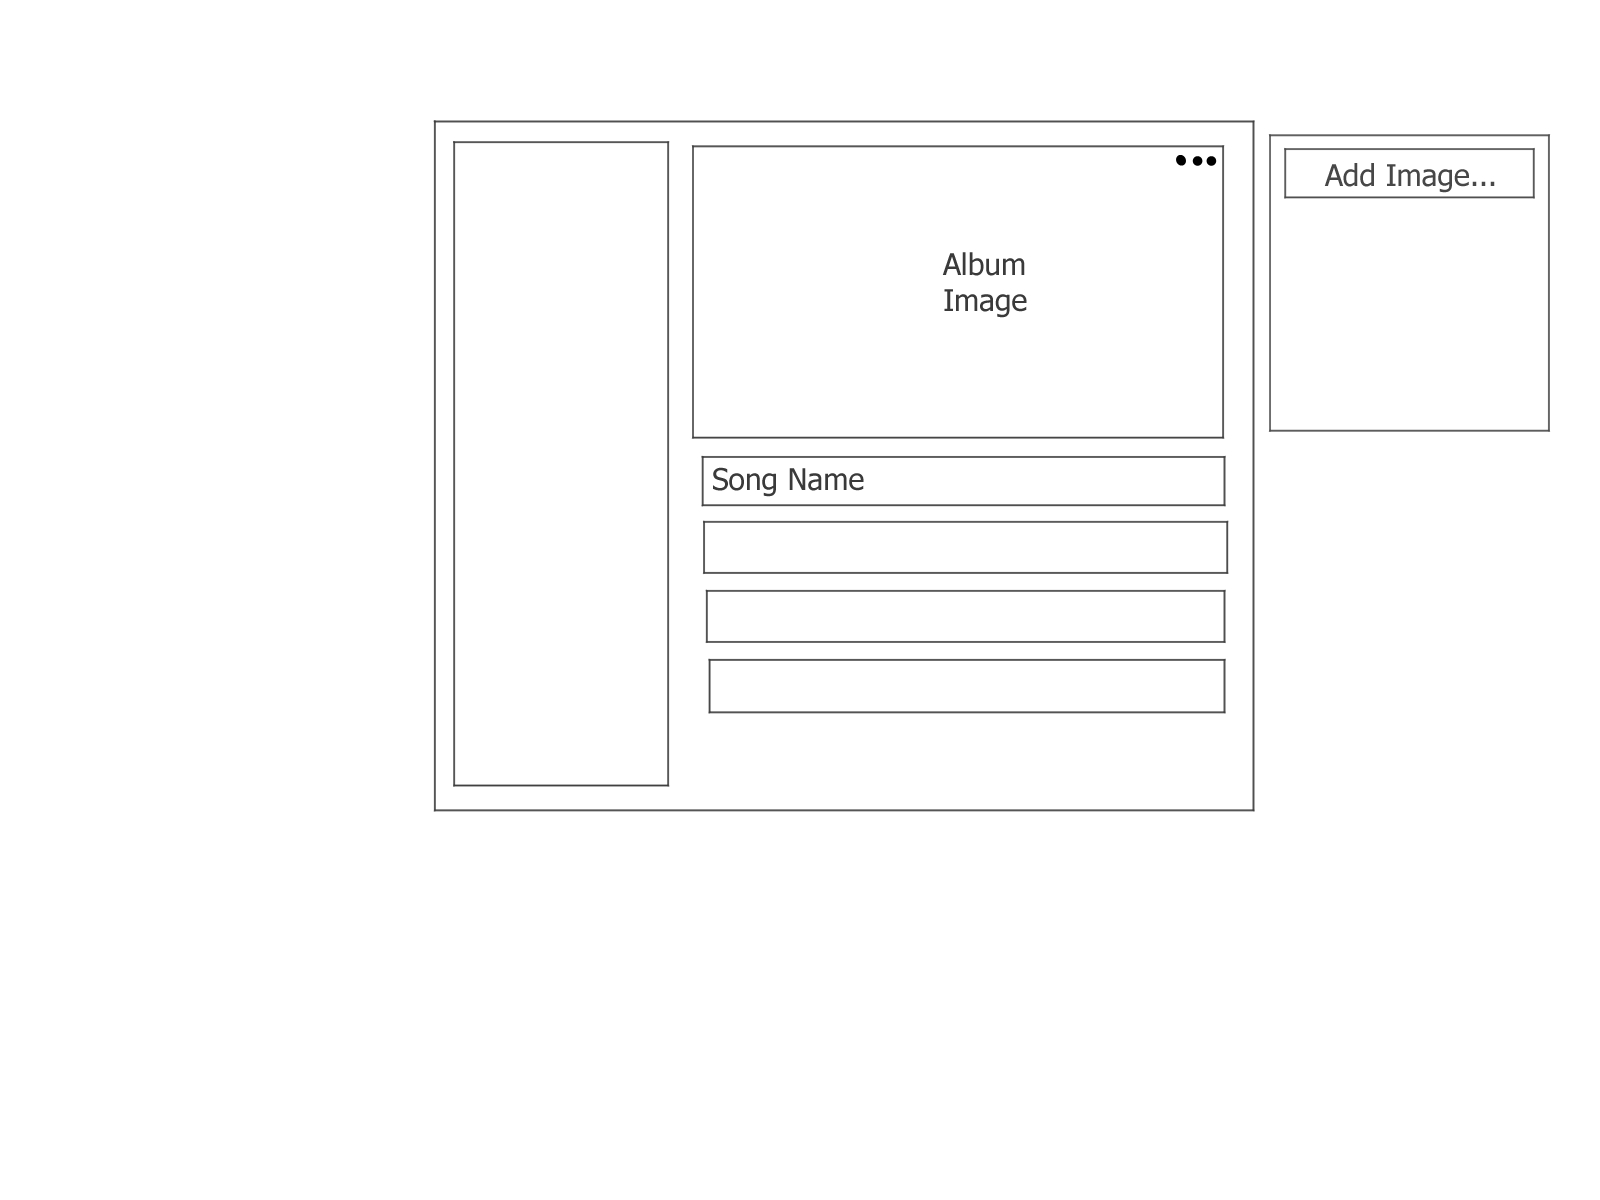
\includegraphics[height=250px, width=350px]{Add_Image_Mock_Up.jpg}
\caption{Use Case 3, Adding album art}
\label{AddAlbumArt}
\end{figure}

\begin{figure}
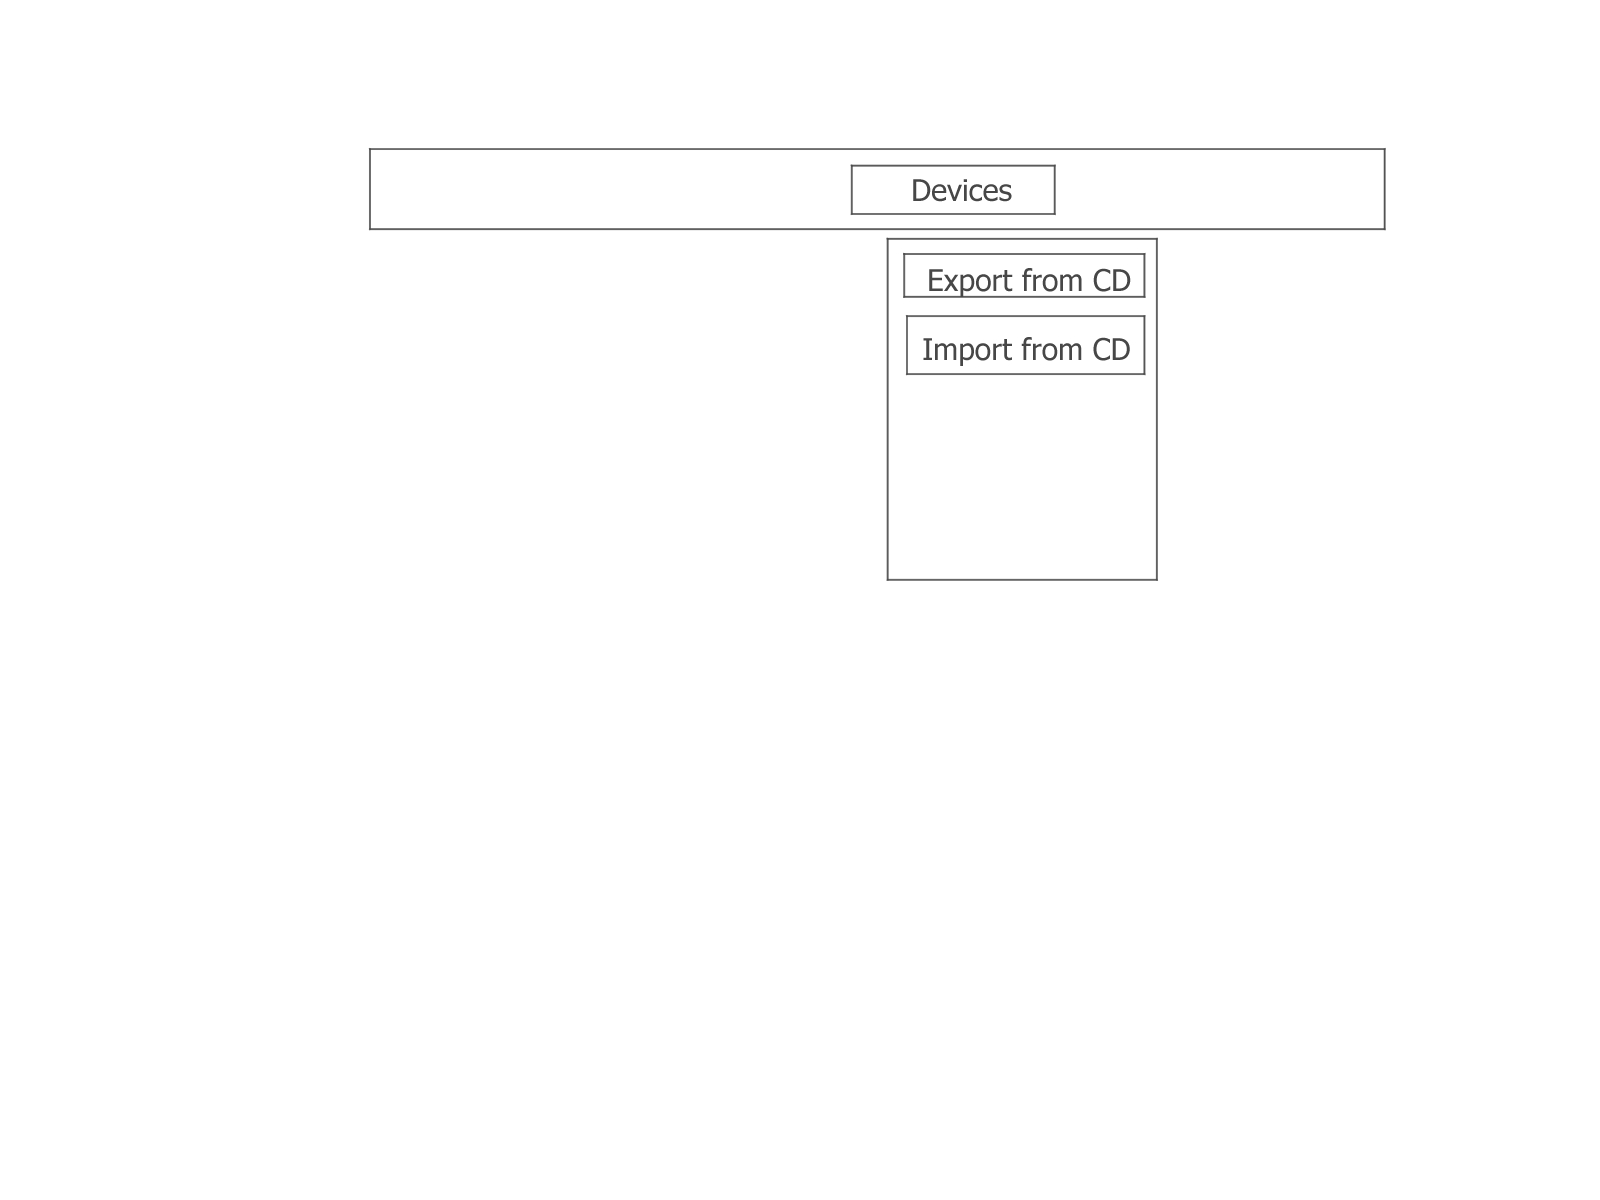
\includegraphics[height=250px, width=350px]{Play_CD_Mock_Up.jpg}
\caption{Use Case 4, Interacting with CD}
\label{PlayCD}
\end{figure}

\begin{figure}
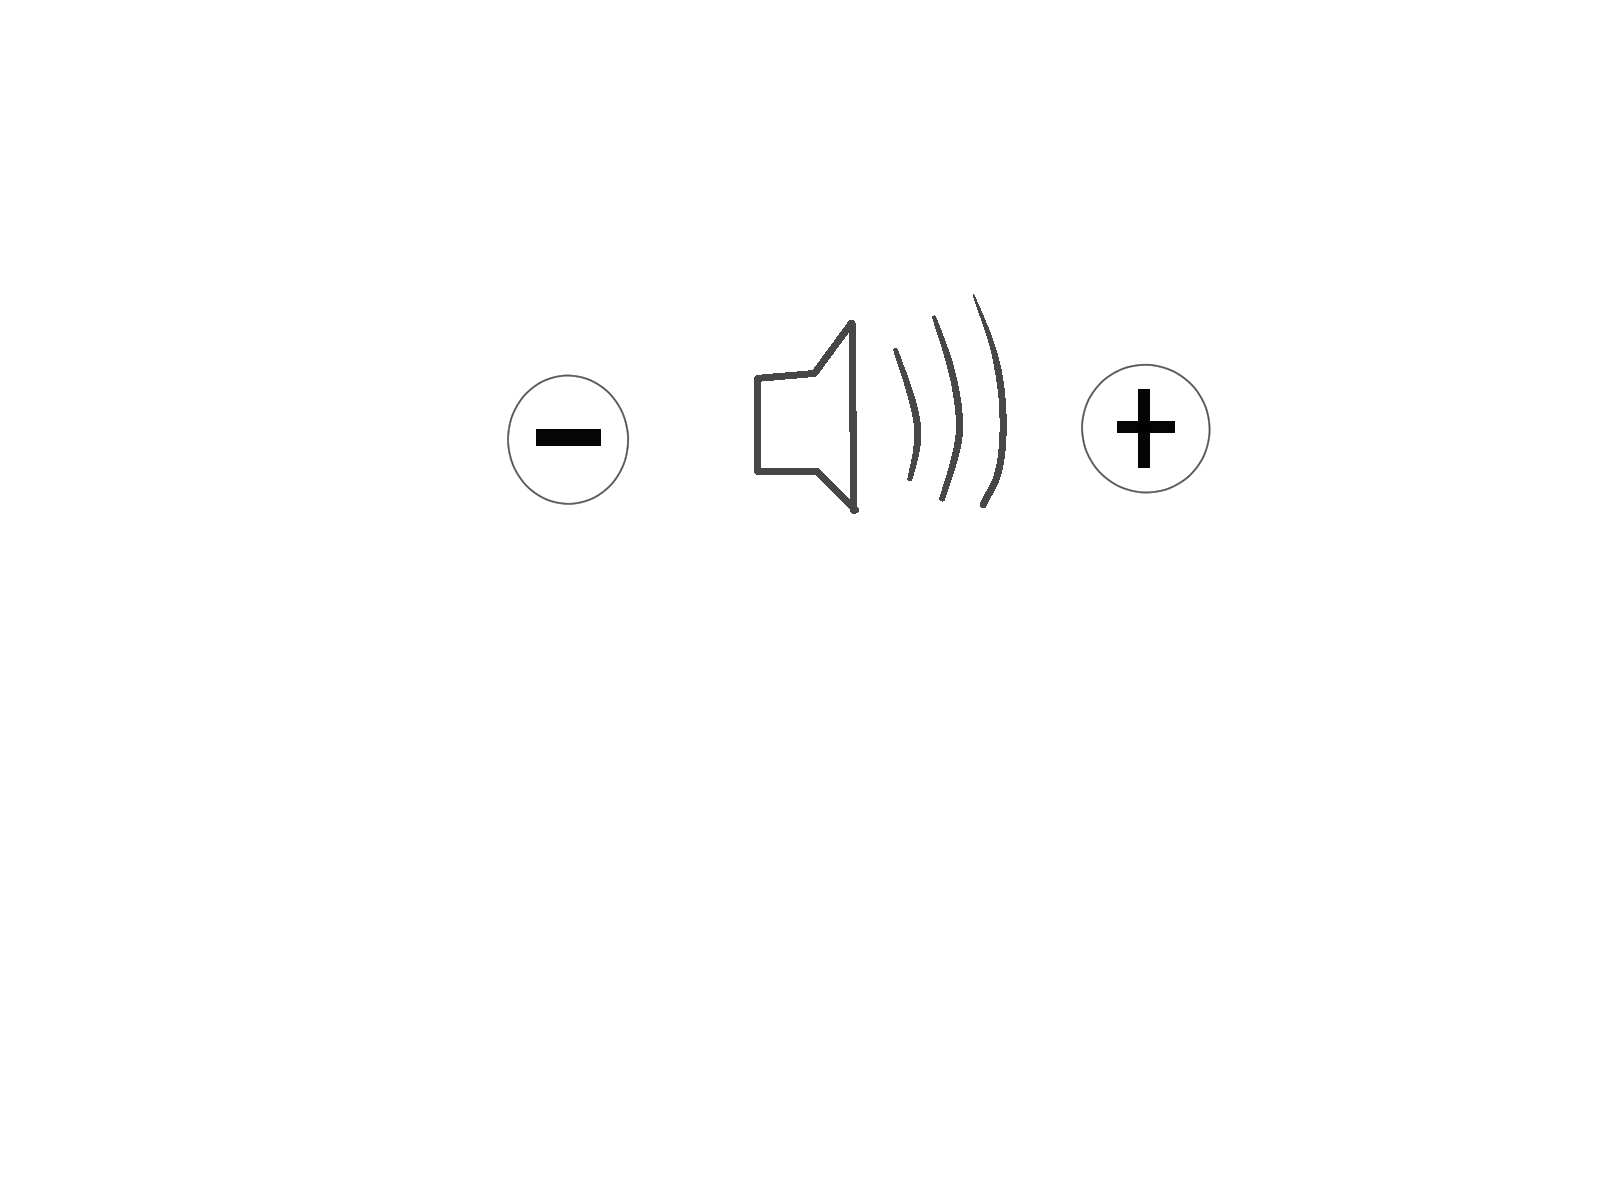
\includegraphics[height=250px, width=250px]{Volume_Button_Mock_Up.jpg}
\caption{Use Case 5, Volume button}
\label{VolumeButton}
\end{figure}

\section{Project Timeline}
Go back to your notes and look up a typical project development life cycle for the Waterfall approach.  How will you follow this life cycle over the remainder of this semester?  This will usually involve a chart showing your proposed timeline, with specific milestones plotted out.  Make sure you have deliverable dates from the course schedule listed, with a plan to meet them (NOTE: these are generally optimistic deadlines).

\section{Project Structure}
At first, this will be a little empty (it will need to be filled in by the time you turn in your final report).  This is your chance to discuss all of your design decisions (consider this the README's big brother).

\subsection{UML Outline}
Show the full structure of your program.  Make sure to keep on updating this section as your project evolves (you often start out with one plan, but end up modifying things as you move along).  As a note, while Dia fails miserably at generating pdfs (probably my fault), I have had much success with png files.  Make sure to wrap your images in a \texttt{figure} environment, and to reference with the \texttt{ref} command.  For example, see Figure \ref{cat2}.

\begin{figure}[ht!]
\includegraphics[scale=1.5]{cat2.jpg}
\caption{Your figures should be in the \emph{figure} environment, and have captions.  Should also be of diagrams pertaining to your project, not random internet kittens}
\label{cat2}
\end{figure}


\subsection{Design Patterns Used}
Make sure to actually use at least 2 design patterns from this class.  This is not normally part of such documentation, but largely just specific to this class -- I want to see you use the patterns!


\section{Results}
This section will start out a little vague, but it should grow as your project evolves.  With each deliverable you hand in, give me a final summary of where your project stands.  By the end, this should be a reflective section discussing how many of your original goals you managed to attain/how many desired use cases you implemented/how many extra features you added.

\subsection{Future Work}
Where are you going next with your project?
For early deliverables, what are your next steps?  (HINT: you will typically want to look back at your timeline and evaluate: did you meet your expected goals?  Are you ahead of schedule?  Did you decide to shift gears and implement a new feature?)
By the end, what do you plan on doing with this project?  Will you try to sell it?  Set it on fire?  Link to it on your resume and forget it exists?




\begin{thebibliography}{1}

\bibitem{IEEEhowto:kopka}
H.~Kopka and P.~W. Daly, \emph{A Guide to \LaTeX}, 3rd~ed.\hskip 1em plus
  0.5em minus 0.4em\relax Harlow, England: Addison-Wesley, 1999.

\end{thebibliography}



\begin{IEEEbiography}{Michael Shell}
Biography text here.
\end{IEEEbiography}

% if you will not have a photo at all:
\begin{IEEEbiographynophoto}{John Doe}
Biography text here.
\end{IEEEbiographynophoto}

% insert where needed to balance the two columns on the last page with
% biographies
%\newpage

\begin{IEEEbiographynophoto}{Jane Doe}
Biography text here.
\end{IEEEbiographynophoto}





% that's all folks
\end{document}


